\section{Schritt 2}
Im Rahmen des zweiten Schrittes kam zum ersten Mal Gurobi zum Einsatz. Ziel der Aufgabe war es hierbei, das Optimierungsproblem für (Formel hier einfügen), über eine Schnittstelle zum Gurobi-Solver, zu lösen. \\
Die Lösung des Optimierungsproblems erfolgt über eine Schnittstelle zum eingebundenen Gurobi-Solvers. Notwendig für diese Optimierung ist jedoch zunächst das Erstellen eines Models. Elementar ist hierbei, dass dem Model Grenzen übermittelt werden. Diese Grenzen ergeben sich in diesem Ansatz aus der eingangs, siehe Schritt 1, berechneten Matrix $A_{k,q}$. Sind diese Constraints ermittelt, wird im Anschluss der Optimierungsprozess angestoßen. \\
Ist die Optimierung erfolgreich, wird im Anschluss daran die optimierte Matrix ausgegeben.

\begin{figure}[h!]
	\centering
	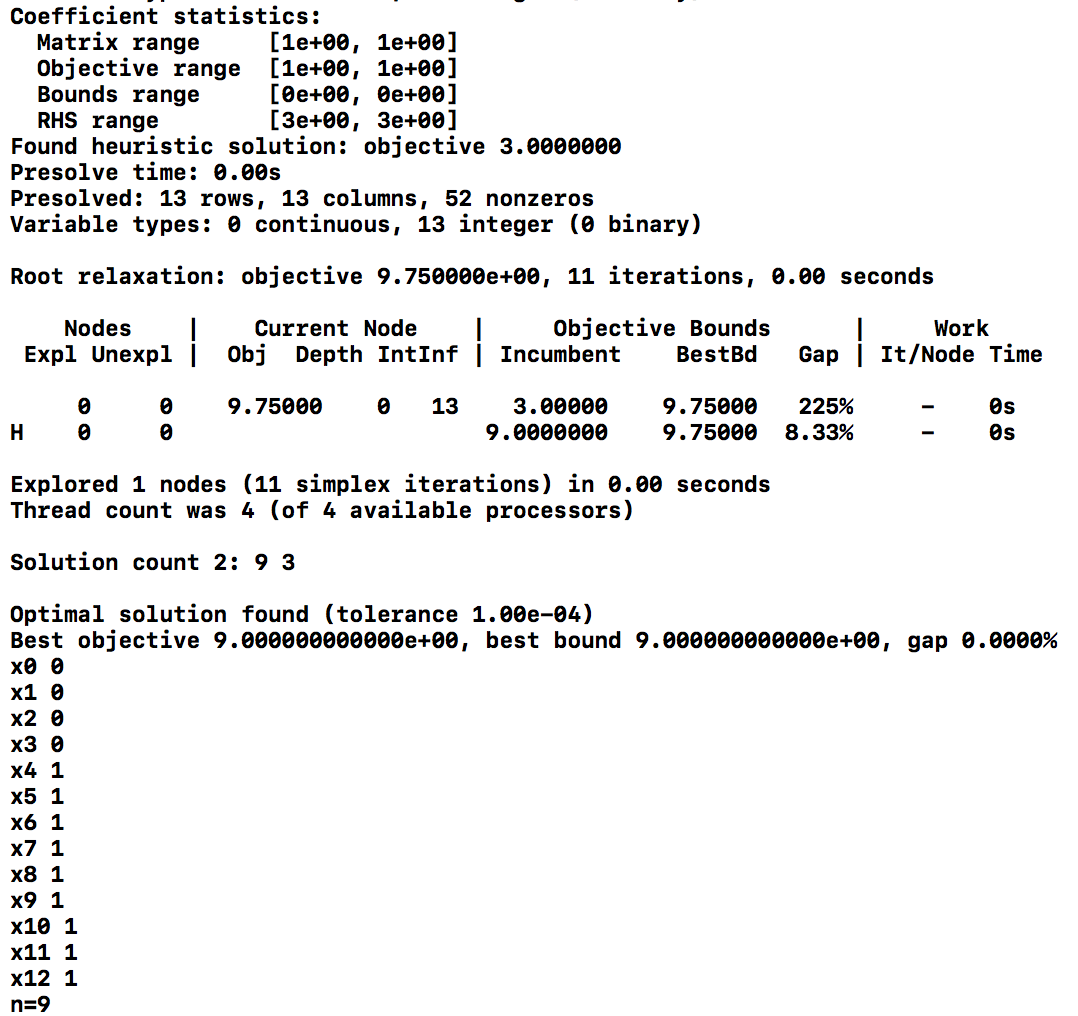
\includegraphics[width=0.5\textwidth]{Pictures/step2_3_3_3}
	\caption{Optimierung für q,k,b=3}
\end{figure}
\newpage